\section{Lo que responde PRIME4API}
\label{sec:limites:prime4api}

Dos de los cálculos de la Sección~\ref{sec:limites:geometrica}, la restricción activa y el tiempo mínimo $t_{\min}$, corresponden a operaciones de PRIME4API, el motor de análisis de la capacidad de Gavira Sánchez \citep{gavira2026tfm}, que las resuelve para cada valor del factor $k$.
Se han ejecutado contra el motor como servicio REST en local, sobre las ocho Datasheets, con la petición y la respuesta de cada pregunta archivadas en el repositorio de datos.
Sus respuestas coinciden con el cálculo a mano salvo por tres convenciones de conteo, por los volúmenes contratados que la Datasheet no declara y por el caudal que toma en Mailgun.
El motor no pasa a correos la cuota diaria en peticiones de MailerSend, y sobre la Datasheet de Mailchimp Transactional no responde a la pregunta del tiempo mínimo.

\subsection{Correspondencia con el cálculo a mano}

La restricción activa a consumo uniforme corresponde a la operación que comprueba si una demanda con \textit{rate} y cuota puede sostenerse durante un período.
El tiempo mínimo $t_{\min}$ de la Ecuación~\eqref{eq:limites-rates} corresponde a la que calcula cuánto tarda en agotarse una cuota, y es lo que Gavira Sánchez llama umbral de agotamiento \citep{gavira2026tfm}.

El factor de equilibrio $k^{*} = Q/(R \cdot W)$ es el número de destinatarios por petición con el que el \textit{rate} y la cuota se agotan a la vez.
Una de las diez preguntas de análisis de Gavira Sánchez pide el CRF con el que dos cuotas de un mismo plan o \textit{pricing} se agotan a la vez \citep{gavira2026tfm}.
Aquí se aplica al par \textit{rate} y cuota, tratando el \textit{rate} como un límite con ventana de un segundo.
El motor no calcula $k^{*}$ con una operación propia: devuelve el tiempo de agotamiento de cada límite para cada $k$, y $k^{*}$ se deriva de esos tiempos.

El factor de equilibrio es el inverso del cociente $R \cdot W / Q$ de las Tablas~\ref{tab:limites-rates} y~\ref{tab:limites-rates-b}, así que se lee en ellas sin otro cálculo.
Vale 0,0019 en Resend Pro, $1{,}9 \cdot 10^{-6}$ en SendGrid Essentials 50K, 0,00096 en MailerSend Hobby y 0,0023 en el entorno de pruebas de Amazon SES.
Como $k$ cuenta destinatarios y no baja de uno, un $k^{*}$ menor que uno significa que la cuota se agota siempre antes que el \textit{rate}.
Las dos tablas tienen una sola fila con cociente menor que uno, MailerSend Starter 1M con la cuenta bajo revisión del proveedor, y su $k^{*}$ es 2,31.
Ningún plan publicado con la cuenta en estado sano tiene un $k \geq 1$ que iguale los dos límites.

Mailgun sí tiene un $k^{*}$ mayor que uno, pero se da entre sus dos contadores de caudal y no entre caudal y cuota.
Con los 2.000.000 de destinatarios y las 80.000 peticiones por ventana que devuelve su cabecera (Sección~\ref{sec:limites:publicado}), el contador de destinatarios corta antes a partir de 25 destinatarios por petición.
En Mailchimp Transactional la operación no se puede plantear, porque el caudal ya está en correos y $k$ no multiplica nada.

El motor reproduce el cálculo a mano en Resend y SendGrid, con tres convenciones propias.
Cuenta la primera ráfaga en $t = 0$, y por eso da 4.999 segundos en Resend Pro donde a mano salen 5.000.
Abre la ventana siguiente en el instante final de un intervalo, y en $t = 30$ días suma ya la primera ráfaga de esa ventana.
Aplica a cada ventana mensual, y no solo a la primera, la cuota ampliada con el sobrecoste que paga el presupuesto.

Aparte de esas convenciones, el motor solo ve el primer volumen contratado de cada plan, porque la Datasheet no declara más.
Con 50 USD al mes, en Resend Pro y SendGrid Essentials el motor parte del volumen de 50.000 correos y da 83.343 y 83.115 correos, cifras correctas para lo que la Datasheet declara.
Los dos proveedores venden un segundo volumen contratado de 100.000 correos por 35 y 34,95 USD, que la Datasheet solo recoge en el registro de procedencia.
Con ese segundo volumen el mismo presupuesto daría 116.000 y 116.722 correos, de modo que el motor se queda entre un 28 y un 29~\% por debajo por un dato que la Datasheet no declara.

En Brevo y Amazon SES las respuestas del motor solo difieren del cálculo a mano por las tres convenciones.
En Mailgun el motor aplica a la vez la cifra por IP que la Datasheet declara en el plan, 1.500 peticiones por segundo, y el contador de la cabecera del envío, 80.000 peticiones por ventana, y calcula con la primera, más baja.
La Tabla~\ref{tab:limites-rates-b} usa solo el contador, dividido entre diez segundos.
En Mailchimp Transactional no responde a la pregunta del tiempo mínimo para enviar 100.000 correos.

El motor aplica una regla de herencia: suma los límites del plan a los del \textit{endpoint}.
Si la cuota y el \textit{rate} de SendGrid Essentials 50K se declaran en el plan y otra vez en el \textit{endpoint}, con $k = 1.000$ el motor da 100.000 correos a 30 días donde el proveedor publica 50.000.
Por eso las Datasheets del catálogo declaran cada límite una sola vez, en el plan si vale para todos los \textit{endpoints} y en el \textit{endpoint} si es propio.
El validador de formato de este trabajo, el que comprueba los tipos y las referencias de cada Datasheet, falla cuando un límite se repite.
La Figura~\ref{fig:capacidad} es la que devuelve el motor sobre las Datasheets con esa regla aplicada.

\subsection{«No publicado» frente a «sin límite» desde el motor}

Antes de adoptar las 5.000 peticiones por segundo de la cabecera, la Datasheet de Postmark tenía vacío el bloque de los \textit{rates}, \texttt{max\_power}, y muestra qué hace el motor en ese caso.
Con el bloque vacío, el motor responde 0 segundos para agotar la cuota de 10.000 correos del plan Basic.
Para 100.000 correos responde 270 días, que son nueve renovaciones de la cuota mensual, como si el \textit{rate} fuese infinito.
Con el caudal de 5.000 peticiones por segundo medido en la cabecera de respuesta, el motor responde 1 segundo para agotar la cuota (2 a mano, por la convención de la primera ráfaga).
Para los 100.000 correos responde 270 días y 1 segundo.

Con un presupuesto de $10^{9}$ USD, la capacidad a un mes pasa de $1{,}1 \cdot 10^{12}$ correos, que solo acota ese presupuesto porque ningún caudal frena el consumo, a 12.960.005.000.
Esa segunda capacidad es $R \cdot W$ más la primera ráfaga de la ventana siguiente.
Ante un pico de 20.000 correos en una hora, el veredicto es negativo en los cuatro planes, tanto con el bloque vacío como con el caudal declarado.
Lo que cambia es la causa que el motor declara: \texttt{rate\_exceeded} con el bloque vacío, aunque lo que se viola es la cuota, y \texttt{quota\_exceeded} con el caudal declarado.

Tratar como infinito el caudal que el esquema deja vacío es la confusión entre «no publicado» y «sin límite» que la propuesta P-04 quiere impedir con una marca explícita de valor no publicado junto al campo (Apartado~\ref{subsec:evolucion:p04}).

En Amazon SES el plan no cambia la respuesta del motor.
Los cuatro planes devuelven 200 correos al día, una petición por segundo, 1.401 correos en siete días y 6.001 al mes, todo tomado del estado \texttt{sandbox}, el entorno de pruebas.
Ante el mismo pico de 20.000 correos en una hora, el motor responde que no en los cuatro planes con la causa \texttt{rate\_exceeded}.
Aquí la causa es correcta, porque una petición por segundo no sostiene los 5,56 correos por segundo que pide la demanda, y la violación se produce desde el instante cero.

\subsection{Los dos regímenes del sobrecoste}

La pregunta del tiempo mínimo para enviar 100.000 correos tiene dos respuestas en el motor, según reciba o no un presupuesto.
Sin el parámetro \texttt{max\_budget}, el motor trata la cuota con sobrecoste como un corte estricto, que no se puede superar pagando: cuenta renovaciones y mide el tiempo en meses.
En MailerSend Hobby, 100.000 correos tardan así 570 días y 41 minutos, que son diecinueve renovaciones de la cuota de 5.000 correos.
Con un presupuesto que no limita, el motor expande la cuota con el sobrecoste que publica el proveedor, y el tiempo lo fija el caudal: 13 horas y 53 minutos.
Esa cifra no aplica la cuota diaria de 1.000 peticiones del plan, que el motor no pasa a correos (Apartado~\ref{subsec:evolucion:h1}): con ella, los 100.000 correos con $k = 1$ tardan 99 días y 8 minutos.

Los dos tiempos salen de datos del proveedor, y ninguno es una hipótesis de este trabajo.
El segundo tampoco exige elegir un presupuesto, porque a partir de lo que cuestan los 100.000 correos la respuesta deja de cambiar.
En Hobby, 100.000 correos cuestan 149,50 USD: con 149,40 USD el motor sigue respondiendo en días, y con 149,50 USD responde 13 horas y 53 minutos, igual que con mil millones.

La Tabla~\ref{tab:a06-presupuesto} pone los dos regímenes al lado en siete APIs.
En Mailgun Basic el presupuesto baja el tiempo de 100.000 correos de 270 días a 1 minuto y 6 segundos.
Ese tiempo sale del caudal de 1.500 peticiones por segundo por IP que declara la Datasheet, y no del contador de 80.000 peticiones por ventana de unos diez segundos.
En Brevo Starter y en Amazon SES la misma llamada no mueve un segundo, porque sus cuotas no declaran sobrecoste.
La distancia entre las dos columnas llega a seis órdenes de magnitud en Postmark Basic con $k = 1$, de 270 días a 19 segundos.

\begin{table}[H]
\centering
\small
\begin{tabular}{|l|c|r|r|}
\hline
\textbf{API y plan} & \textbf{$k$} & \textbf{Corte estricto} & \textbf{Presupuesto que no limita} \\
\hline
Postmark Basic          & 1     & 270 d 1 s            & 19 s \\
                        & 50    & 270 d                & 0 s \\
\hline
Resend Pro              & 1     & 30 d 1 h 23 min 19 s & 2 h 46 min 39 s \\
                        & 50    & 30 d 1 min 39 s      & 3 min 19 s \\
\hline
SendGrid Essentials 50K & 1     & 30 d 4 s             & 9 s \\
                        & 1.000 & 30 d                 & 0 s \\
\hline
MailerSend Hobby        & 1     & 570 d 41 min         & 13 h 53 min \\
                        & 70    & 570 d                & 11 min \\
\hline
Brevo Starter           & 1     & 570 d 4 s            & 570 d 4 s \\
                        & 2.000 & 570 d                & 570 d \\
\hline
SES Pro (\texttt{sandbox}) & 1  & 499 d 3 min 19 s     & 499 d 3 min 19 s \\
                        & 50    & 499 d 3 s            & 499 d 3 s \\
\hline
Mailgun Basic           & 1     & 270 d 6 s            & 1 min 6 s \\
                        & 1.000 & 270 d                & 0 s \\
\hline
\end{tabular}
\caption[Tiempo mínimo para 100.000 correos con corte estricto y con presupuesto que no limita]{Tiempo mínimo para enviar 100.000 correos en un plan de pago de cada API, respondido por PRIME4API \citep{prime4apirepo} en los dos regímenes. Sin \texttt{max\_budget}, la cuota con sobrecoste se trata como corte estricto y el motor cuenta renovaciones. Con un presupuesto que no limita, el motor la expande y manda el caudal. Brevo y SES son los dos casos sin sobrecoste declarado, y por eso las dos columnas coinciden. Las filas de SES son las del estado \texttt{sandbox}, el único que el proveedor cifra. Mailchimp Transactional no aparece porque el motor no responde a esta pregunta sobre su Datasheet. La fila de Mailgun usa el caudal de 1.500 peticiones por segundo por IP. La fila de MailerSend Hobby no aplica la cuota diaria de 1.000 peticiones del plan (Apartado~\ref{subsec:evolucion:h1}).}
\label{tab:a06-presupuesto}
\end{table}

Nada en la Datasheet dice cuál de los dos regímenes describe el plan.
La cuota lleva su sobrecoste, pero no declara si el proveedor lo cobra sin más, si exige aprobarlo o si lo limita un tope.
El tope de sobrecoste de SendGrid, diez veces el volumen del plan (500.000 correos en Essentials 50K), tendría que entrar en la operación que calcula el importe del sobrecoste, pero la Datasheet no tiene dónde declararlo.
La propuesta P-07, que añade a la cuota un campo para ese tope, lo permite (Apartado~\ref{subsec:evolucion:p07}).
El modo del sobrecoste no tiene campo: es la carencia F-13 de la Tabla~\ref{tab:sinforma}, vista ahora desde el motor, y sigue entre las carencias sin forma fijada.

\subsection{La cuota que no cambia de unidad}
\label{subsec:evolucion:h1}

MailerSend declara en su plan Hobby dos cuotas en unidades distintas: 5.000 correos al mes y 1.000 peticiones al día.
Su \textit{endpoint} de envío declara un \texttt{workload} de hasta 70 destinatarios por petición, y ese factor $k$ es el que el motor usa para pasar de una unidad a otra.
Pedida la curva en correos, la respuesta trae el caudal y la cuota mensual, y no la diaria.
Pedida en peticiones, trae los tres límites: el caudal y la cuota diaria tal cual, y la mensual dividida por $k$.
De las tres conversiones que el factor permite, el motor hace dos.
Multiplica por $k$ el caudal de peticiones para darlo en correos, y divide por $k$ la cuota mensual de correos para darla en peticiones.
La cuota diaria en peticiones no la lleva a correos.

Que el motor no pase la cuota diaria a correos cambia la respuesta.
Con $k = 1$, el motor responde que los 5.000 correos de Hobby se agotan en 41 minutos, mientras que con la cuota diaria de 1.000 peticiones tardarían 4 días y 8 minutos.
La capacidad a un mes con presupuesto sin tope sale de 5.184.120 correos, y con la cuota diaria sería de 30.000.
Con 50 USD de presupuesto el motor devuelve 33.786,67 correos, sin redondear, y con la cuota diaria también saldrían 30.000.
Quien pregunta en correos, que es la unidad del dominio, recibe la cifra optimista.
La Figura~\ref{fig:limites:hobby-peticiones} es la misma llamada pedida en peticiones, y en ella la cuota diaria sí aparece: la curva sube 1.000 cada medianoche durante cinco días.

\begin{figure}[H]
\centering
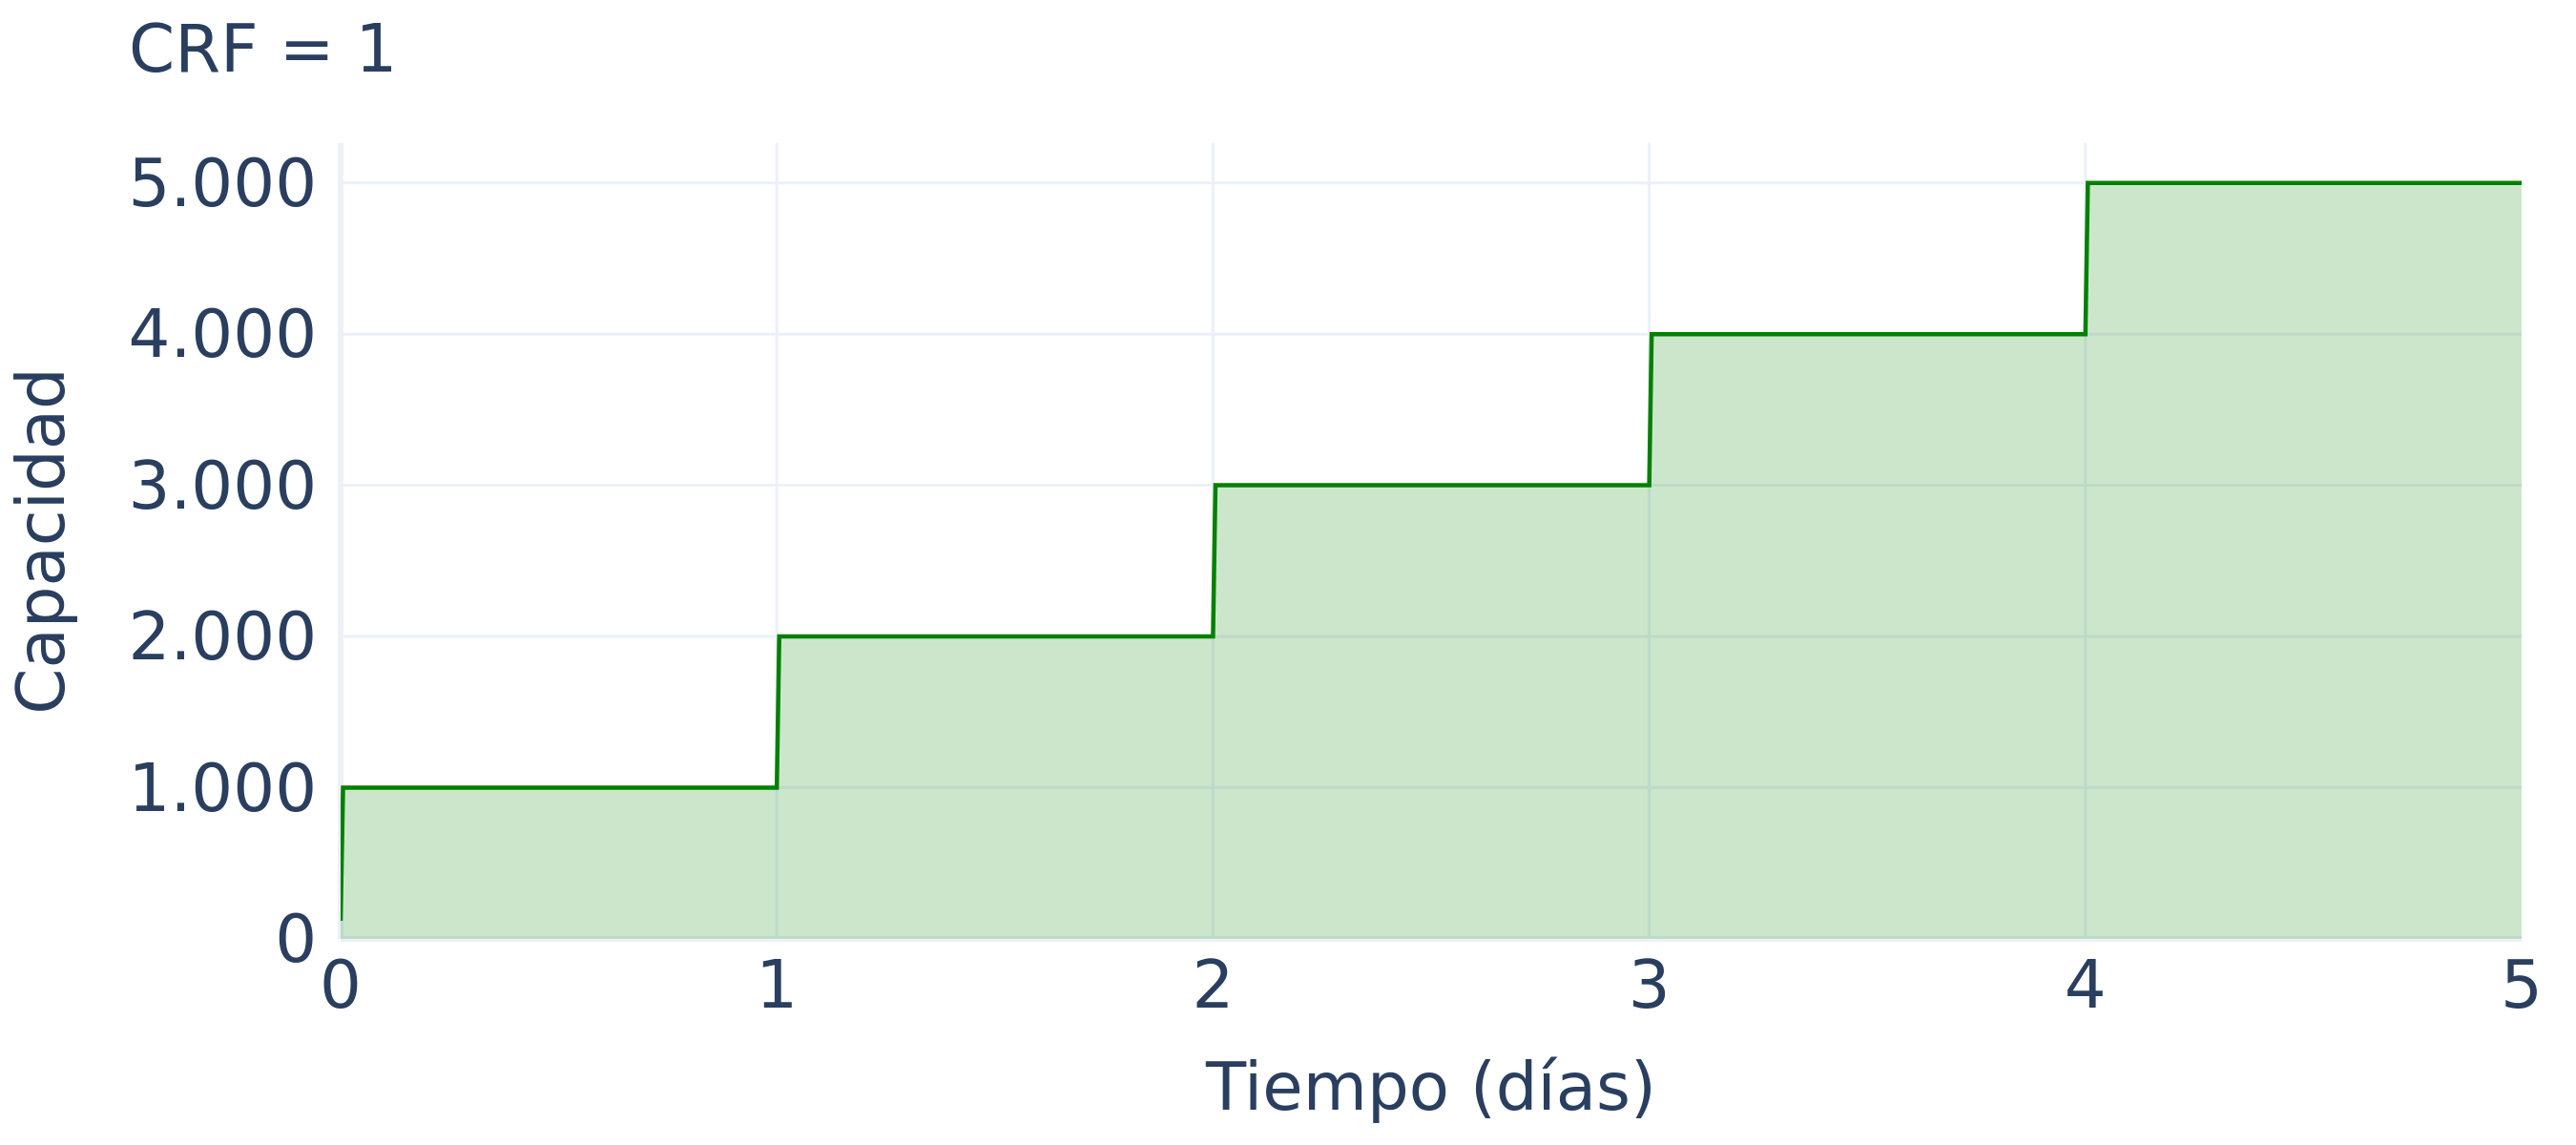
\includegraphics[width=0.72\textwidth]{fig/capacidad_mailersend_hobby_k1_peticiones_2026-10-25.png}
\caption[Curva de capacidad de MailerSend Hobby en peticiones]{Curva de capacidad de MailerSend Hobby con $k = 1$ sobre cinco días, pedida a PRIME4API \citep{prime4apirepo} en peticiones. Es la misma llamada que la gráfica (c) de la Figura~\ref{fig:capacidad}, con \texttt{capacity\_unit} en peticiones. La cuota diaria de 1.000 peticiones del plan sí entra, y la curva sube 1.000 cada medianoche UTC hasta los 5.000 de la cuota mensual el quinto día. Con $k = 1$ cada petición lleva un correo, así que la curva se lee también en correos. El tramo de \textit{rate} (120 peticiones por minuto durante ocho minutos) no se distingue a esta escala.}
\label{fig:limites:hobby-peticiones}
\end{figure}

El renderizador del motor oculta las curvas en peticiones.
Si se le pide la gráfica de MailerSend Hobby sin filtrar la unidad, devuelve cuatro figuras y las cuatro son de correos.
La curva en peticiones, la única que lleva la cuota diaria de Hobby, solo se dibuja con el parámetro \texttt{show\_derived\_requests}, cuyo valor por defecto es falso.
El \textit{endpoint} de datos, en cambio, devuelve las dos unidades sin que se le pida, así que la ausencia está solo en el dibujo.

La conversión que falta corresponde al motor.
La Datasheet de MailerSend declara los tres límites con su unidad y el factor $k$ que haría falta, que el motor usa en las otras dos conversiones.
MailerSend es la única de las ocho APIs que declara cuotas en dos unidades, y por eso el problema solo aparece en ella.
El defecto no cambia el plan más barato en ninguna de las tres recomendaciones de presupuesto del contraste, para 12.000, 25.000 y 40.000 correos.
Queda una pregunta que el catálogo no convierte en propuesta: una Datasheet con límites en dos unidades no declara en cuál mide el plan el proveedor, y quien la consulta elige la unidad al preguntar.

\subsection{Capacidad con un presupuesto menor que el precio del plan}

La operación \texttt{/capacity-at} calcula cuántos correos caben hasta una fecha con un presupuesto dado.
Con un presupuesto menor que el precio del plan, devuelve la cuota base más la primera ráfaga de la ventana siguiente.
En MailerSend Professional con 50 USD responde 50.120 correos y no marca el plan como no asequible, a diferencia de \texttt{/budget/recommendation}, que recomienda planes según el presupuesto y sí lo marca.
SendGrid Pro, que cuesta 89,95 USD al mes, responde 110.000 correos con el mismo presupuesto de 50 USD.

Brevo Professional cuesta 499 USD al mes, y con 50 USD el motor devuelve 151.000 correos con la categoría de caudal General y 152.000 con la Advanced.
Son los 150.000 de la cuota más lo que cabe en el primer segundo de la ventana siguiente, así que la categoría de caudal no cambia el volumen del mes.
En los tres casos el motor no amplía la cuota con sobrecoste, porque el presupuesto no cubre el precio del plan, pero devuelve igualmente la cuota base y no avisa de que el plan no es asequible.
Quien consulta \texttt{/capacity-at} con un presupuesto menor que el precio del plan tiene que cruzar la respuesta con \texttt{/budget/recommendation} para saber si puede pagar el plan.

El contraste cubre las ocho Datasheets del catálogo. Una API con cuotas en tres unidades o con un sobrecoste que exija aprobación previa podría sacar a la luz convenciones del motor que estas ocho no activan.
